\section{Model description and statistical methods}
\subsection{Our Model}
As mentioned in the introduction, we will mostly be investigating the basic model: segregation of $20$ individuals of type $1$ and $20$ individuals of type $2$ on an $8 \times 8$ board.
In this model an individual is considered unhappy if less than \(\frac{1}{3}\) of his/her neighbours shares his/her type. 
If an individual is unhappy, this individual will move to the nearest place where he/she would be happier.
Any person without neighbours is by definition considered unhappy (so his/her happiness is $0$), since people prefer living with others over living alone.
Furthermore, the basic model uses the second order neighbourhood; the maximum number of neighbours a person can have is 8. 
The model however can be changed by preference in several ways.\\

First of all, the board size can be varied.
If no other parameters are altered, this will only imply that the board becomes fuller or emptier.
Secondly, we can change the number of types on the board.
For instance, one can consider a $12\times 12$ board with $10$ types of individuals and $10$ individuals per type: see Figure \ref{fig:example big board}.
As one can see, far more individuals have been moved to another place on the board and segregation takes place.

\vspace{-10pt}
\begin{figure}[H]
	\centering
    \begin{subfigure}{0.45\textwidth}
        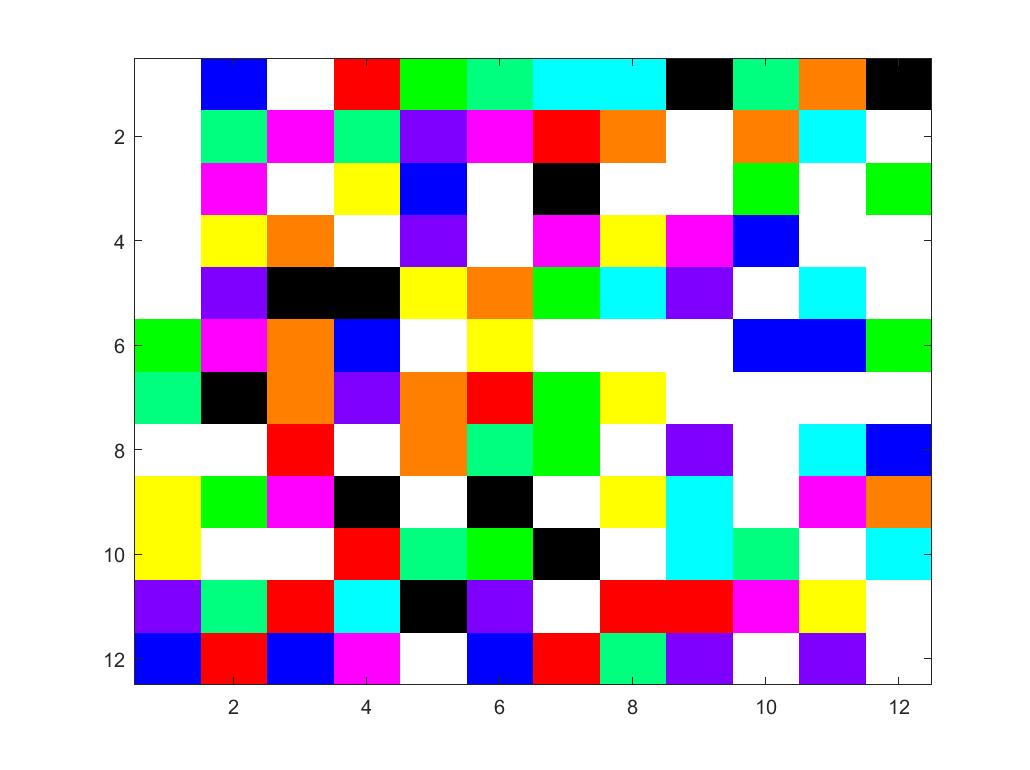
\includegraphics[width=\textwidth]{vb2beginbord.jpg}
        \caption{Situation before segregation}
        \label{fig:example big board begin}
    \end{subfigure}\hspace{0cm}
    ~ 
    \begin{subfigure}{0.45\textwidth}
        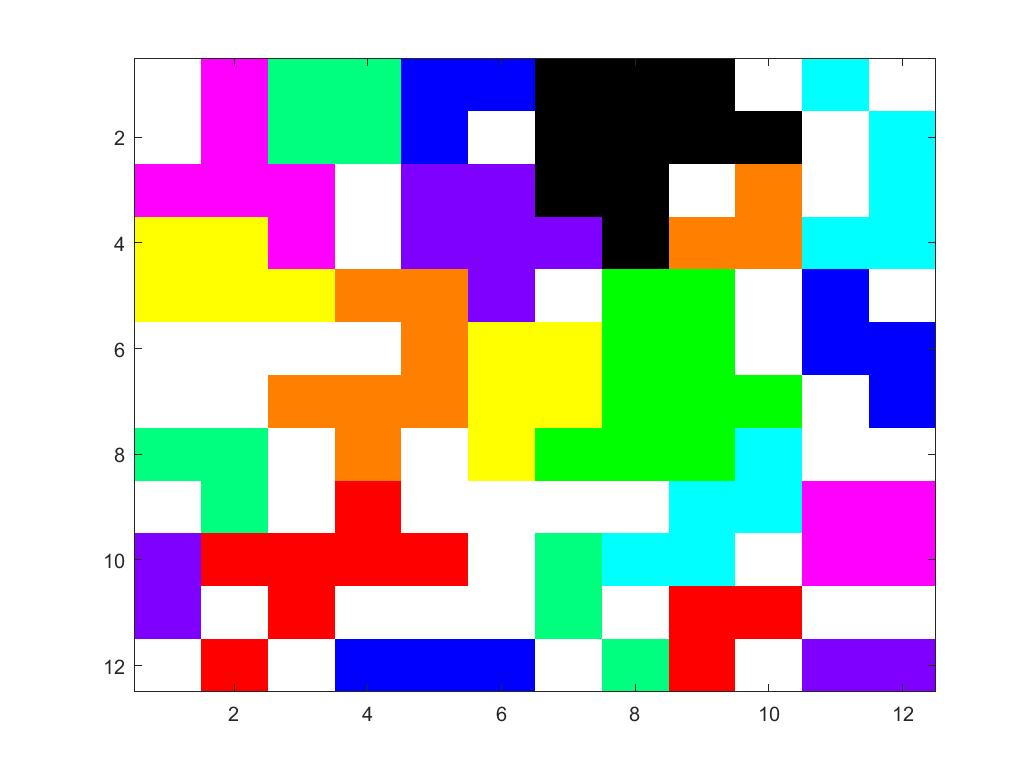
\includegraphics[width=\textwidth]{vb2eindbord.jpg}
        \caption{Situation after segregation}
        \label{fig:example big board end}
    \end{subfigure}
    ~ 
    \vspace{-5pt}
    \caption{An example of segregation on a $12\times 12$ board with $100$ individual of $10$ different types}
    \label{fig:example big board}
\end{figure}
\vspace{-10pt}

Subsesquently, we can vary our 'Happiness Rule': the minimal fraction of neighbours that has to share an individuals type, in order to be considered happy.
The expectation is that the time to reach equilibrium increases as the Happiness Rule is strengthened.
This makes sense as every individual needs to be surrounded by relatively more neighbours of his/her own type.
In consequence, larger homogenous groups will be formed after segregation with a higher Happiness Rule.
In Figures \ref{fig:examplehap2/3} and \ref{fig:examplehap1} the effect of a Happiness Rule of respectively $\frac{2}{3}$ and $1$ on the board after segregation is illustrated.
\vspace{-10pt}
\begin{figure}[H]
	\centering
    \begin{subfigure}{0.4\textwidth}
        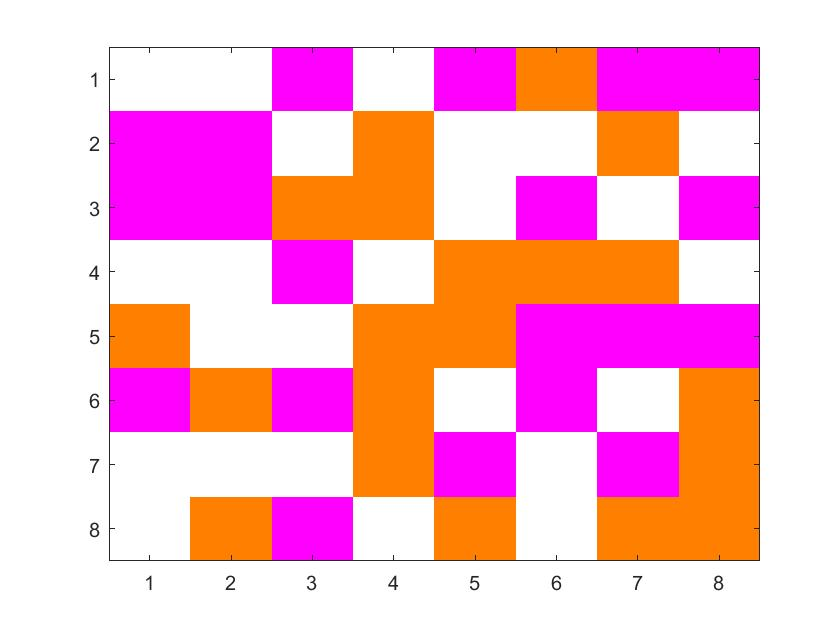
\includegraphics[width=\textwidth]{vb3beginbord.jpg}
        \caption{Situation before segregation}
        \label{fig:example hap 2/3 begin}
    \end{subfigure}\hspace{0cm}
    ~ 
    \begin{subfigure}{0.4\textwidth}
        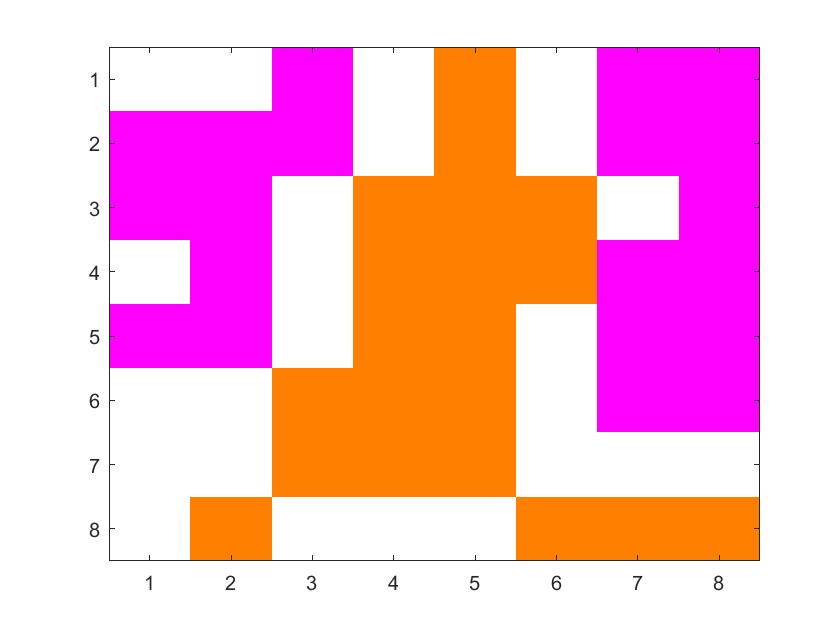
\includegraphics[width=\textwidth]{vb3eindbord.jpg}
        \caption{Situation after segregation}
        \label{fig:example hap 2/3 end}
    \end{subfigure}
    ~ 
    \vspace{-5pt}
    \caption{An example of segregation in a model with Happiness Rule $\frac{2}{3}$}
    \label{fig:examplehap2/3}
\end{figure}

\begin{figure}[H]
	\centering
    \begin{subfigure}{0.4\textwidth}
        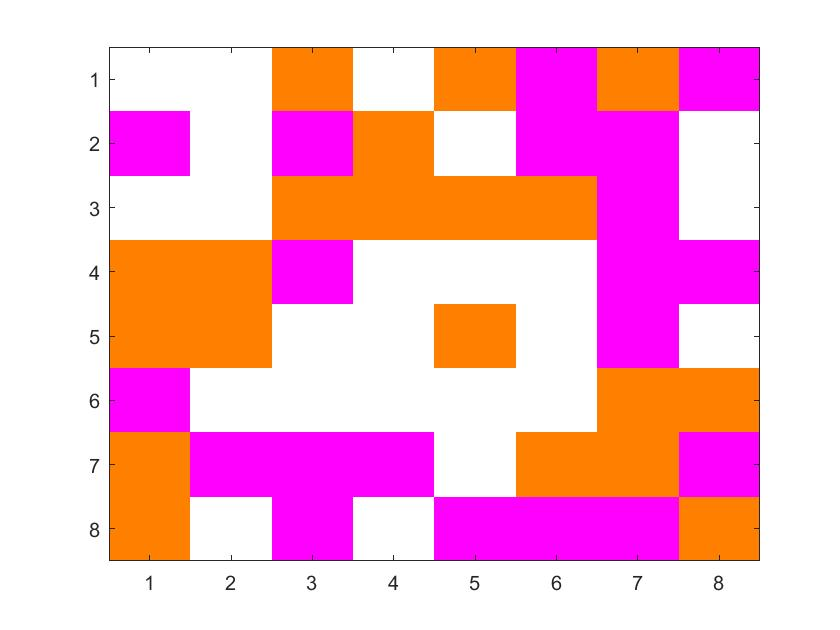
\includegraphics[width=\textwidth]{vb4beginbord.jpg}
        \caption{Situation before segregation}
        \label{fig:example hap 1 begin}
    \end{subfigure}\hspace{0cm}
    ~ 
    \begin{subfigure}{0.4\textwidth}
        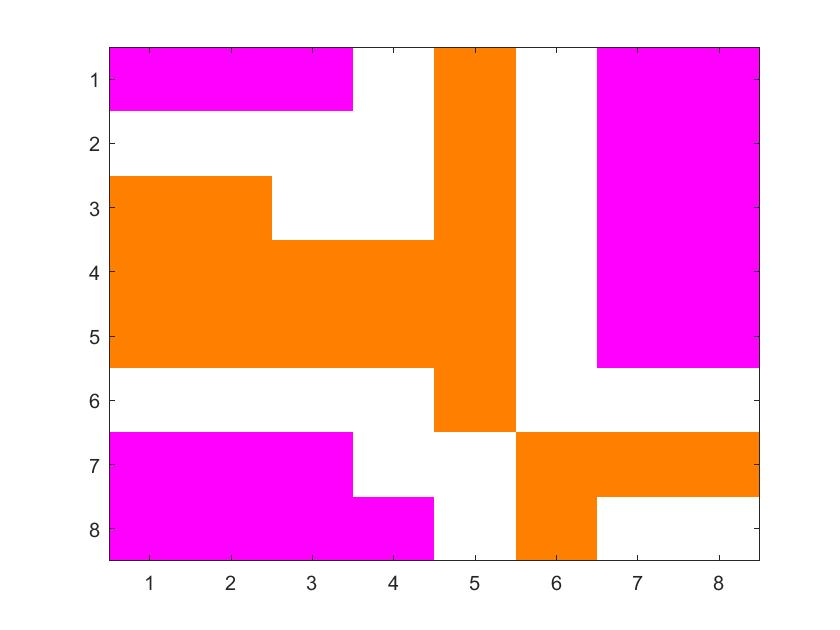
\includegraphics[width=\textwidth]{vb4eindbord.jpg}
        \caption{Situation after segregation}
        \label{fig:example hap 1 end}
    \end{subfigure}
    ~ 
    \vspace{-5pt}
    \caption{An example of segregation in a model with Happiness Rule $1$}
    \label{fig:examplehap1}
\end{figure}

In Figure \ref{fig:example hap 1 end} it is illustrated that every individual lives homogenous if a Happiness Rule of $1$ is applied.
We will elaborate on the effect of the Happiness Rule on the model in sections \ref{sec:aantgen} and \ref{sec:meanhappy}.\\

\begin{wrapfigure}{r}{0.3\textwidth}
\vspace{-20pt}
\centering
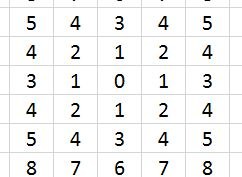
\includegraphics[scale=0.8]{buurtorde.jpg}
\caption{Neighbourhood order}
\vspace{-10pt}
\label{fig:neighbourhood}
\end{wrapfigure}

In addition,  the type of neighbourhood can be changed.
The neighbourhood is  by default a second order neighbourhood, in which both the adjacent and diagonal people are considered neighbours. 
There exists only one smaller type of neighbourhood: the first order neighbourhood. 
Only adjacent neighbours are accounted for this type of neighbourhood; a person has up to four neighbours.
The way the different types of neighbourhood are defined is illustrated in figure \ref{fig:neighbourhood}.
Here, $0$ represents the individual himself and every other place displays which order of  of neighbourhood it belongs to.
We will not examine the effect of the type of neighbourhood on the segregation in our model in this report.
However, some interesting graphs are included in the appendix.\\

Moreover, we included the possibility for individuals to move to a random place on the board if he/she is not happy, rather than moving to the closest position.
In the basic model he/she will move to the nearest place where he/she will become happier. With random displacement, we expect that it takes longer to reach an equilibrium.
As above, we will not discuss the impact of the random displacement in our report, but we added some results in our appendix.\\

Furthermore, we expanded the model with the so-called 'criminals'.
One can choose to have $c$ out of the $n$ individuals behave as if they were a criminal.
Any person who is not a criminal himself, does not like criminals in his neighbourhood, and thus his/her happiness will be $0$, overruling any positive effect of friendly neighbours, if a criminal lives in his/her neighbourhood.
As a result, all criminals should end up living together.
In figure \ref{fig:examplecrim}, one can see an example of the basic model with $10$ criminals among the $40$ individuals.
It is visible that our expectation is not always the outcome.
In this case, equilibrium is reached, because every unhappy individual cannot move to another place, since every empty location is in the neighbourhood of a criminal.
So the unhappy individuals will not become happier on these places.

\begin{figure}[H]
	\centering
    \begin{subfigure}{0.4\textwidth}
        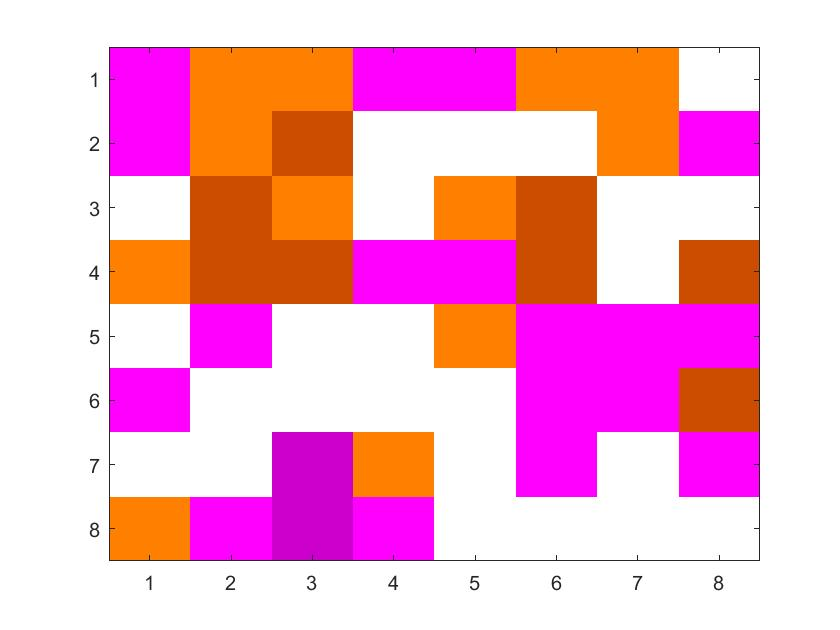
\includegraphics[width=\textwidth]{vb5beginbord.jpg}
        \caption{Situation before segregation}
        \label{fig:example crim begin}
    \end{subfigure}\hspace{0cm}
    ~ 
    \begin{subfigure}{0.4\textwidth}
        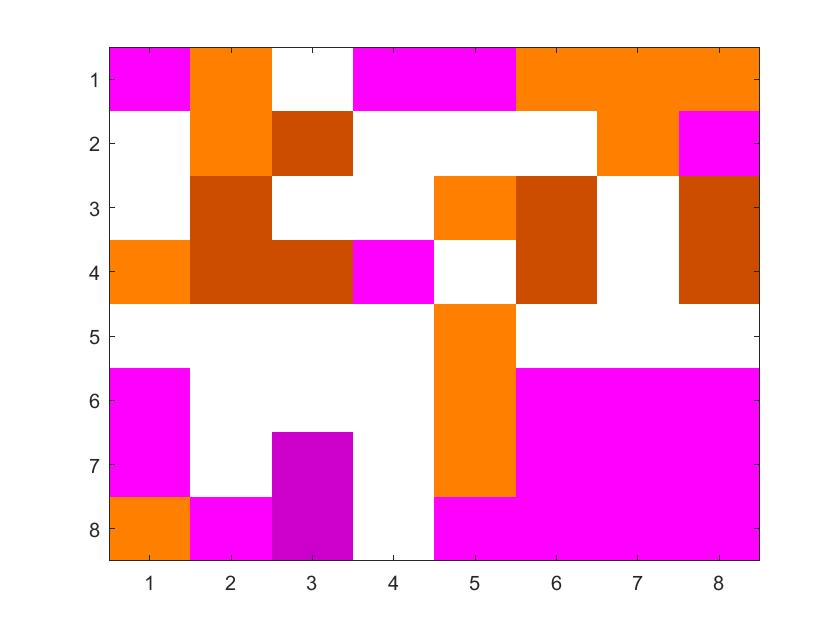
\includegraphics[width=\textwidth]{vb5eindbord.jpg}
        \caption{Situation after segregation}
        \label{fig:example crim end}
    \end{subfigure}
    ~ 
    \caption{An example of segregation in the basic model with a total number of $10$ criminals (the slightly darker places: i.e. the individuals on (3,8) and (3,2))}
    \label{fig:examplecrim}
\end{figure}

Last, we made it possible for individuals to switch to another type.
In our model there are two versions of switching.
The first version is only possible if there are only two different types present on the board.
In this version of switching, every person has a chance $p$ of switching to the other type before he moves.
In the other version, every unhappy individual will switch type depending on the type of his/her neighbours.
This is further elaborated on in section \ref{section:switch}.
Individuals without neighbours will not switch types, since they have no neighbours who extert their influence on them.
We will investigate the effect of the second version of switching further in section \ref{section:switch}.
\subsection{The applied statistical test}
\textbf{The two sample t-test}:\\
For the following sections, we will mostly use the two sample t-test (ttest2) from Matlab for comparing the means of two distributions. We consider two means to be comparable when they are equal. Otherwise, they are not comparable.\\
\\
This t-test tests the null-hypothesis $H_0:\mu=\nu$ with $\mu,\nu$ respectively the mean of the distribution of $X$ and $Y$, against $H_1:\mu\neq\nu$. It uses the test statistics:
 \[T=\frac{\overline{X}-\overline{Y}}{\sqrt{\frac{S^2_X}{m}-\frac{S^2_Y}{n}}}\]
This test assumes that the mean difference $\mu-\nu$ is normally distributed, and since our data are from the discrete random variables, this assumption would not make sense. 
However, according to the central limit theorems, we may make this assumption only for a sufficiently large sample size. 
Although exact calculations are required to determine the sample size, we simply chose a sample size of 5000. In section \ref{subsec:avegensw}, we even chose a sample size of 50000, due to the asymmetric distribution of our data. Also, for simplicity, we usually took $m=n$. Furthermore, we have adjusted the test, such that it does not assume the two data sets have an equal variance for the data distribution (this is achieved by setting 'Vartype' as unequal in Matlab).\\
\\
\textbf{Other tests}:\\
For testing the goodness of fit of our hypothesized distribution in sections \ref{sec:aantgen} and \ref{section:switch}, we have used the two-sample kolomogorov-smirnov test and the chi-squared test in Matlab. More information about these tests can be found on Mathworks.  


